\section{Kết quả thực nghiệm}

\subsection{Kết nối các thiết bị}

\begin{figure}[H]
    \centering
    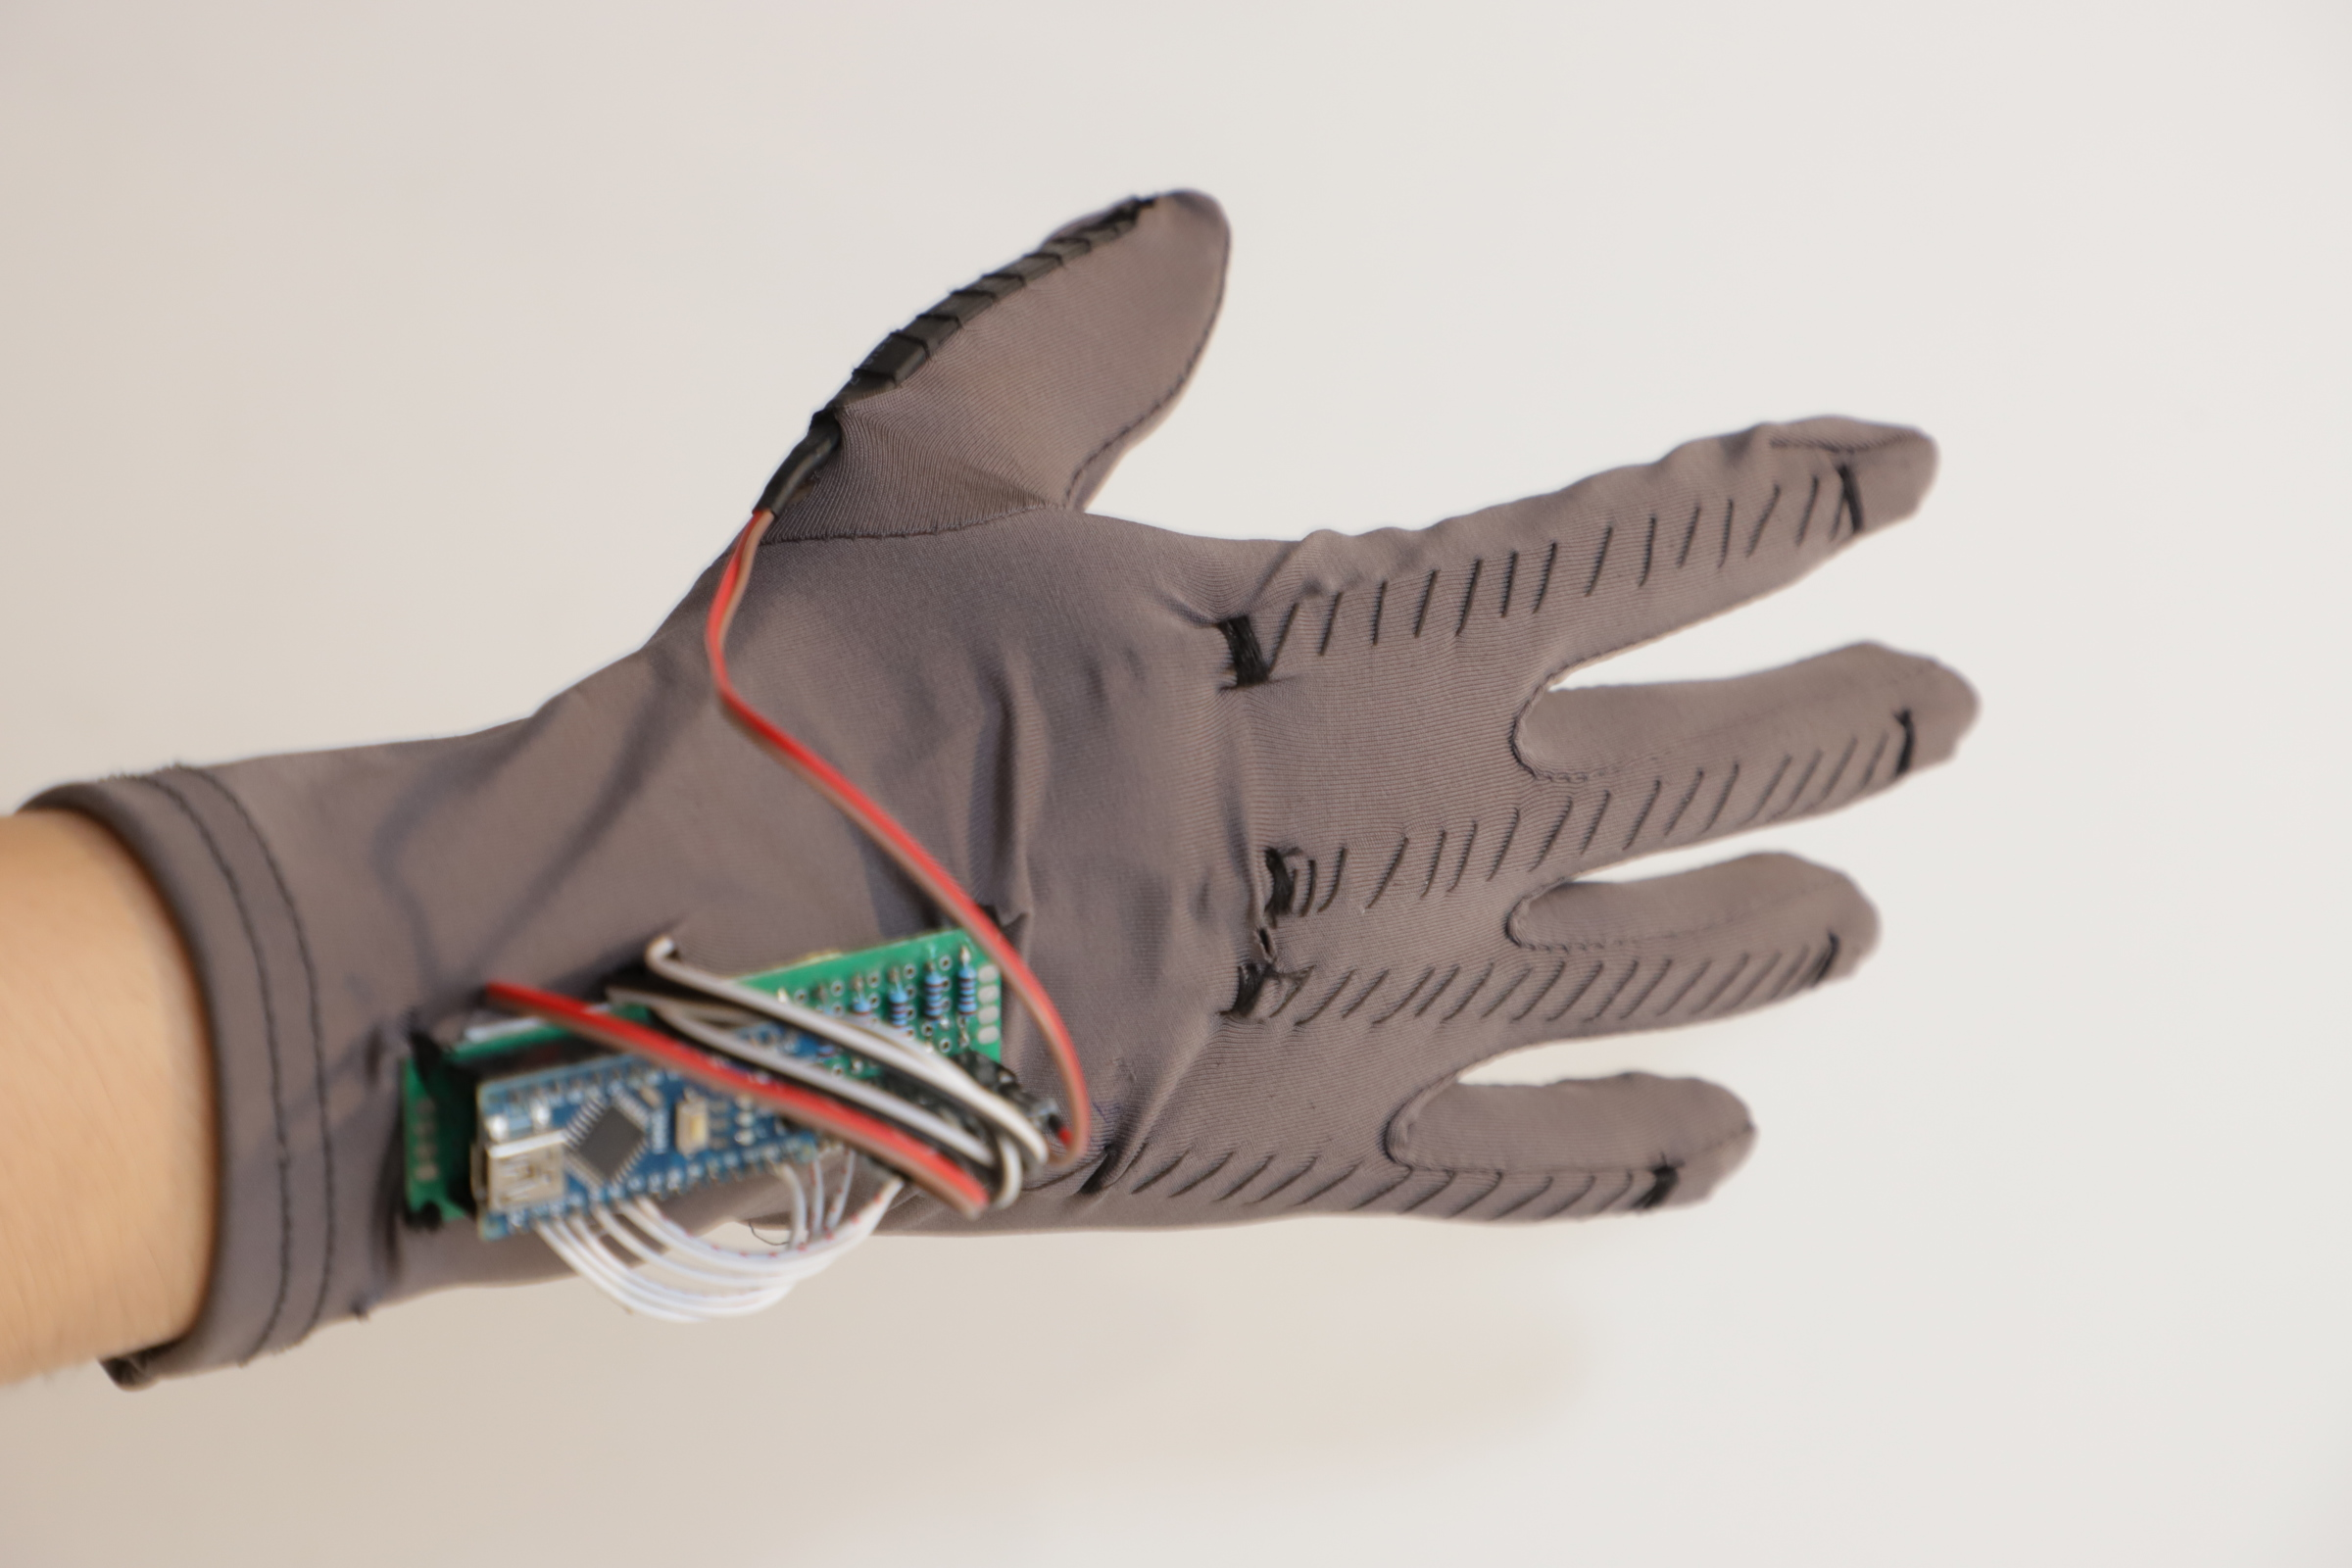
\includegraphics[width=13cm]{Images/Experimental results/overview.JPG}
\caption{Hình sản phẩm 1}
\end{figure}

\begin{figure}[H]
    \centering
    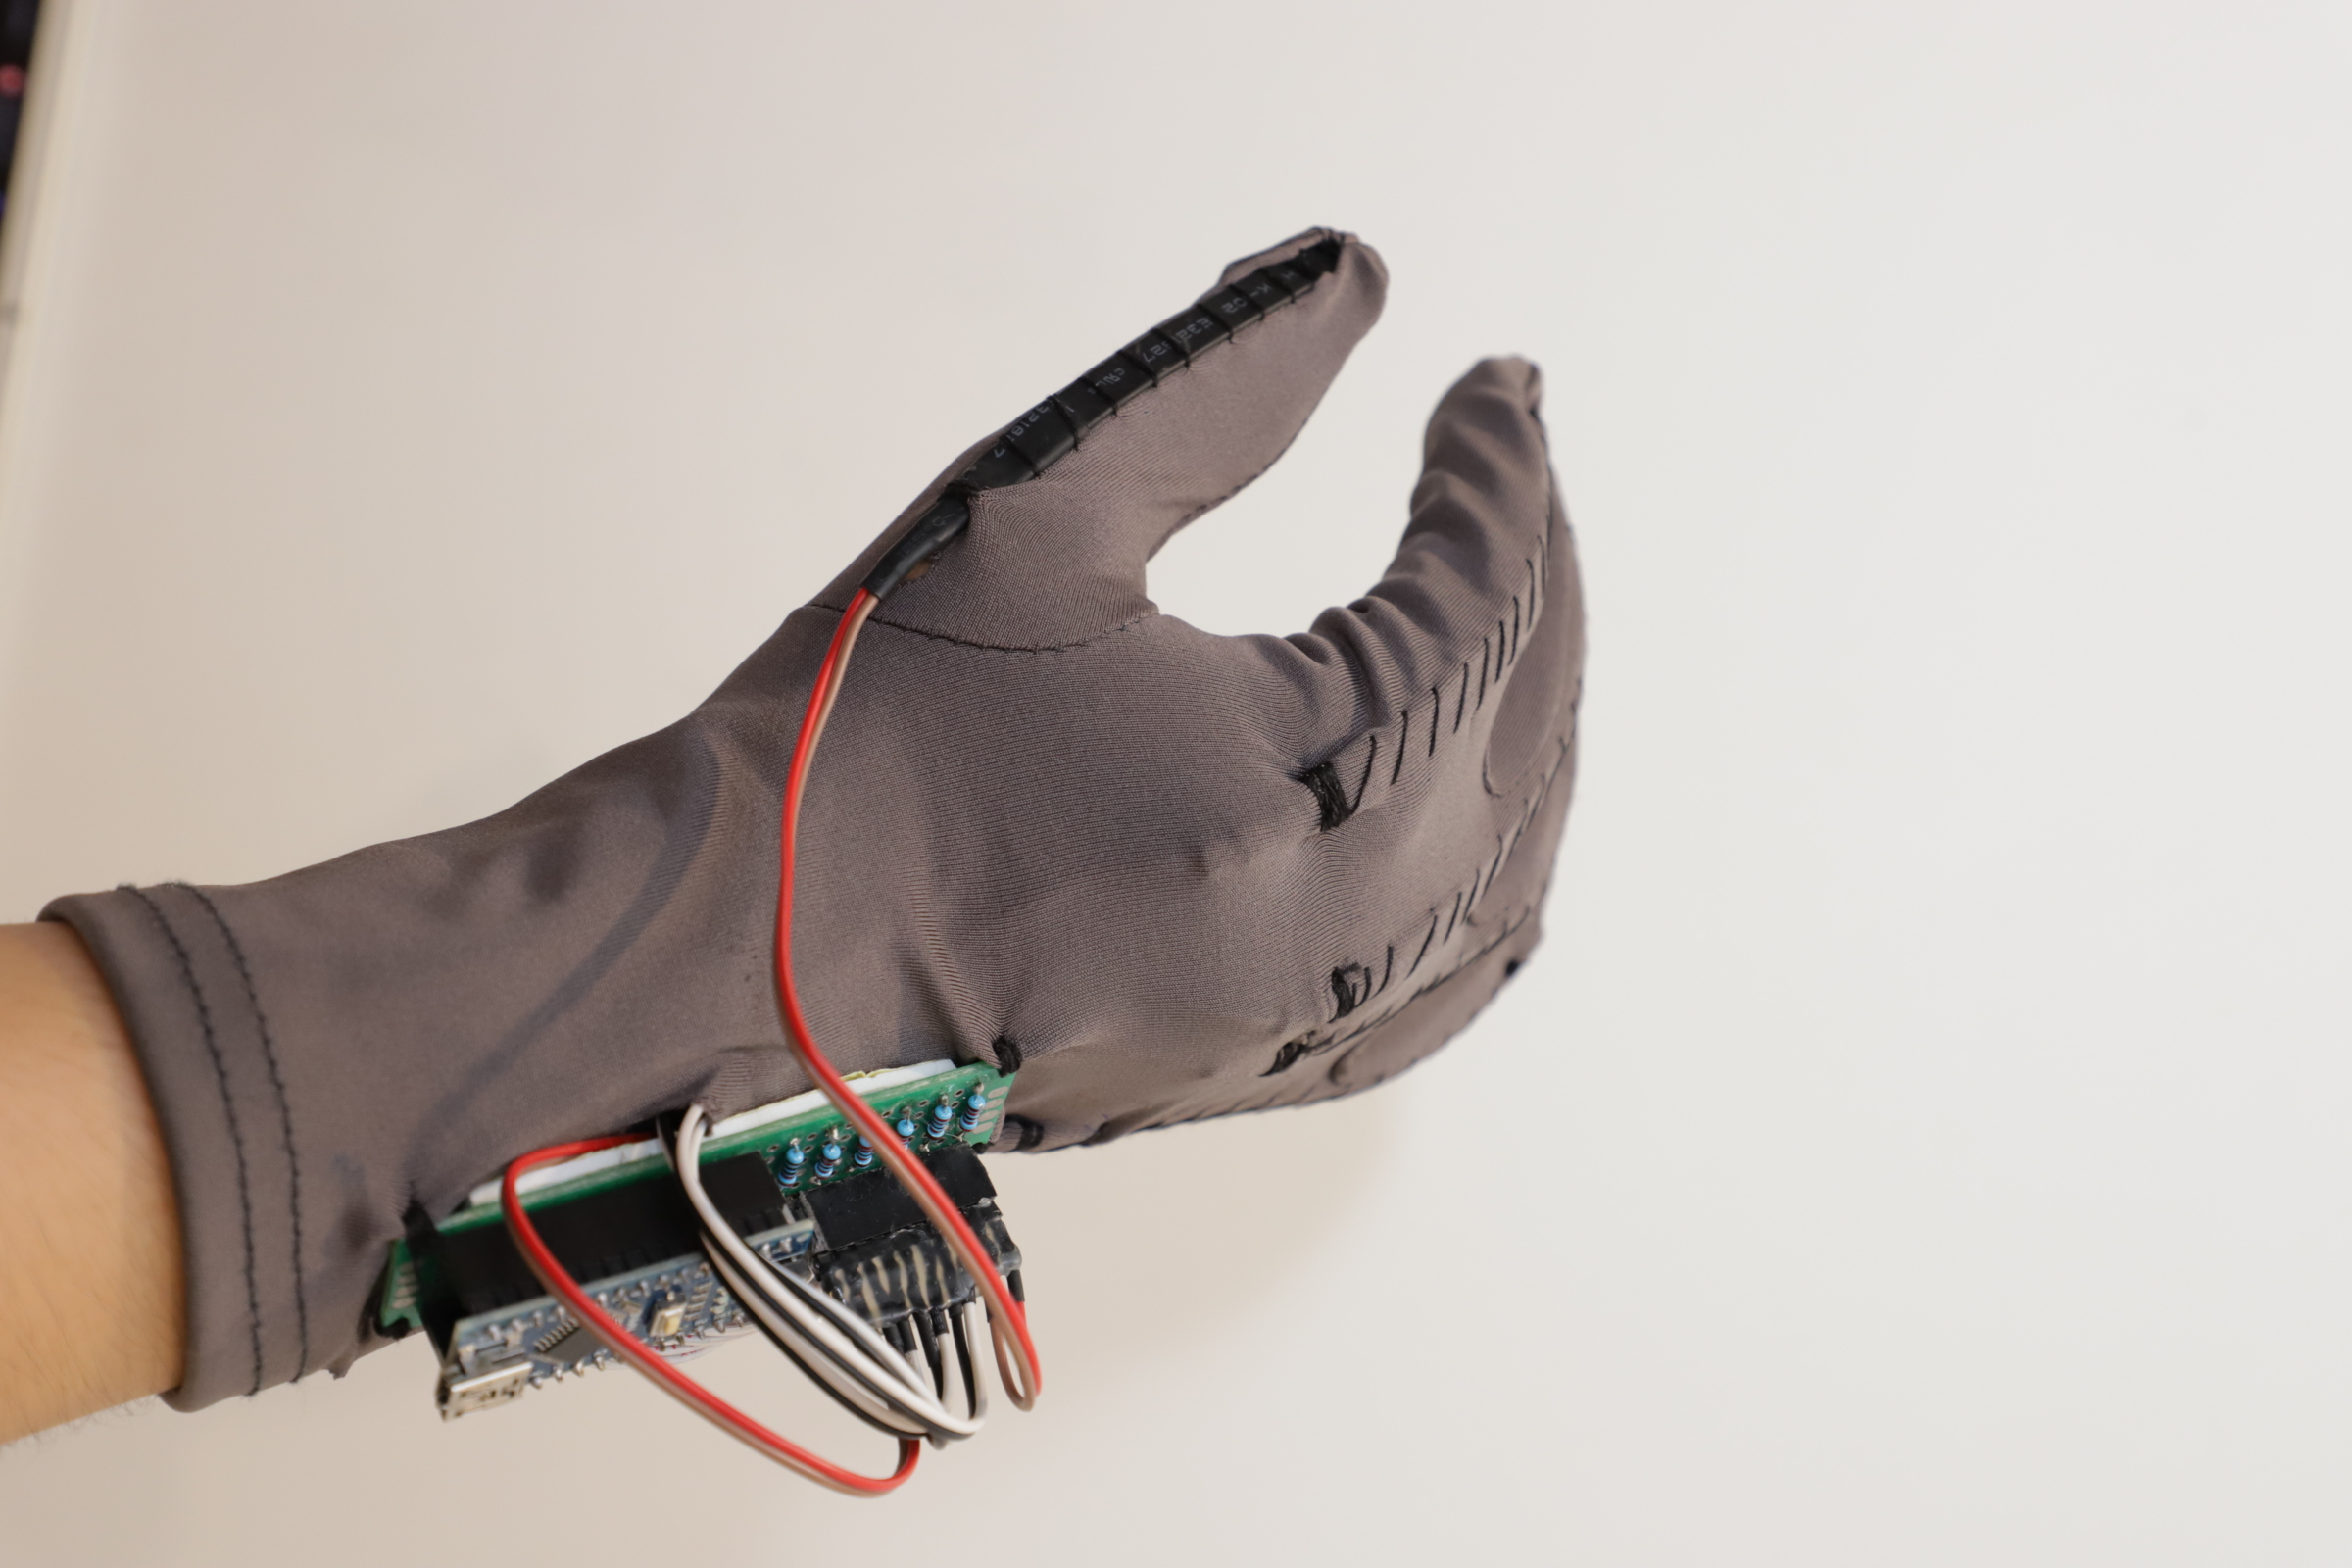
\includegraphics[width=13cm]{Images/Experimental results/overview1.JPG}
\caption{Hình sản phẩm 2}
\end{figure}

\indent Sản phẩm này được thiết kế để theo dõi và đo lường sự uốn cong của ngón tay thông qua việc tích hợp 5 flex sensor vào các ngón tay của chiếc bao tay. Mỗi flex sensor được đặt một cách chính xác và linh hoạt để theo dõi các chuyển động của ngón tay giúp thu thập dữ liệu có độ chính xác cao nhất.

\indent Cụ thể, mỗi ngón tay trên bao tay có một flex sensor được tích hợp, giúp ghi lại mức độ uốn cong của từng ngón. Điều này mang lại khả năng đọc dữ liệu chính xác về độ uốn cong và sự linh hoạt của ngón tay khi người đeo thực hiện các cử động khác nhau.


\begin{figure}[H]
    \centering
    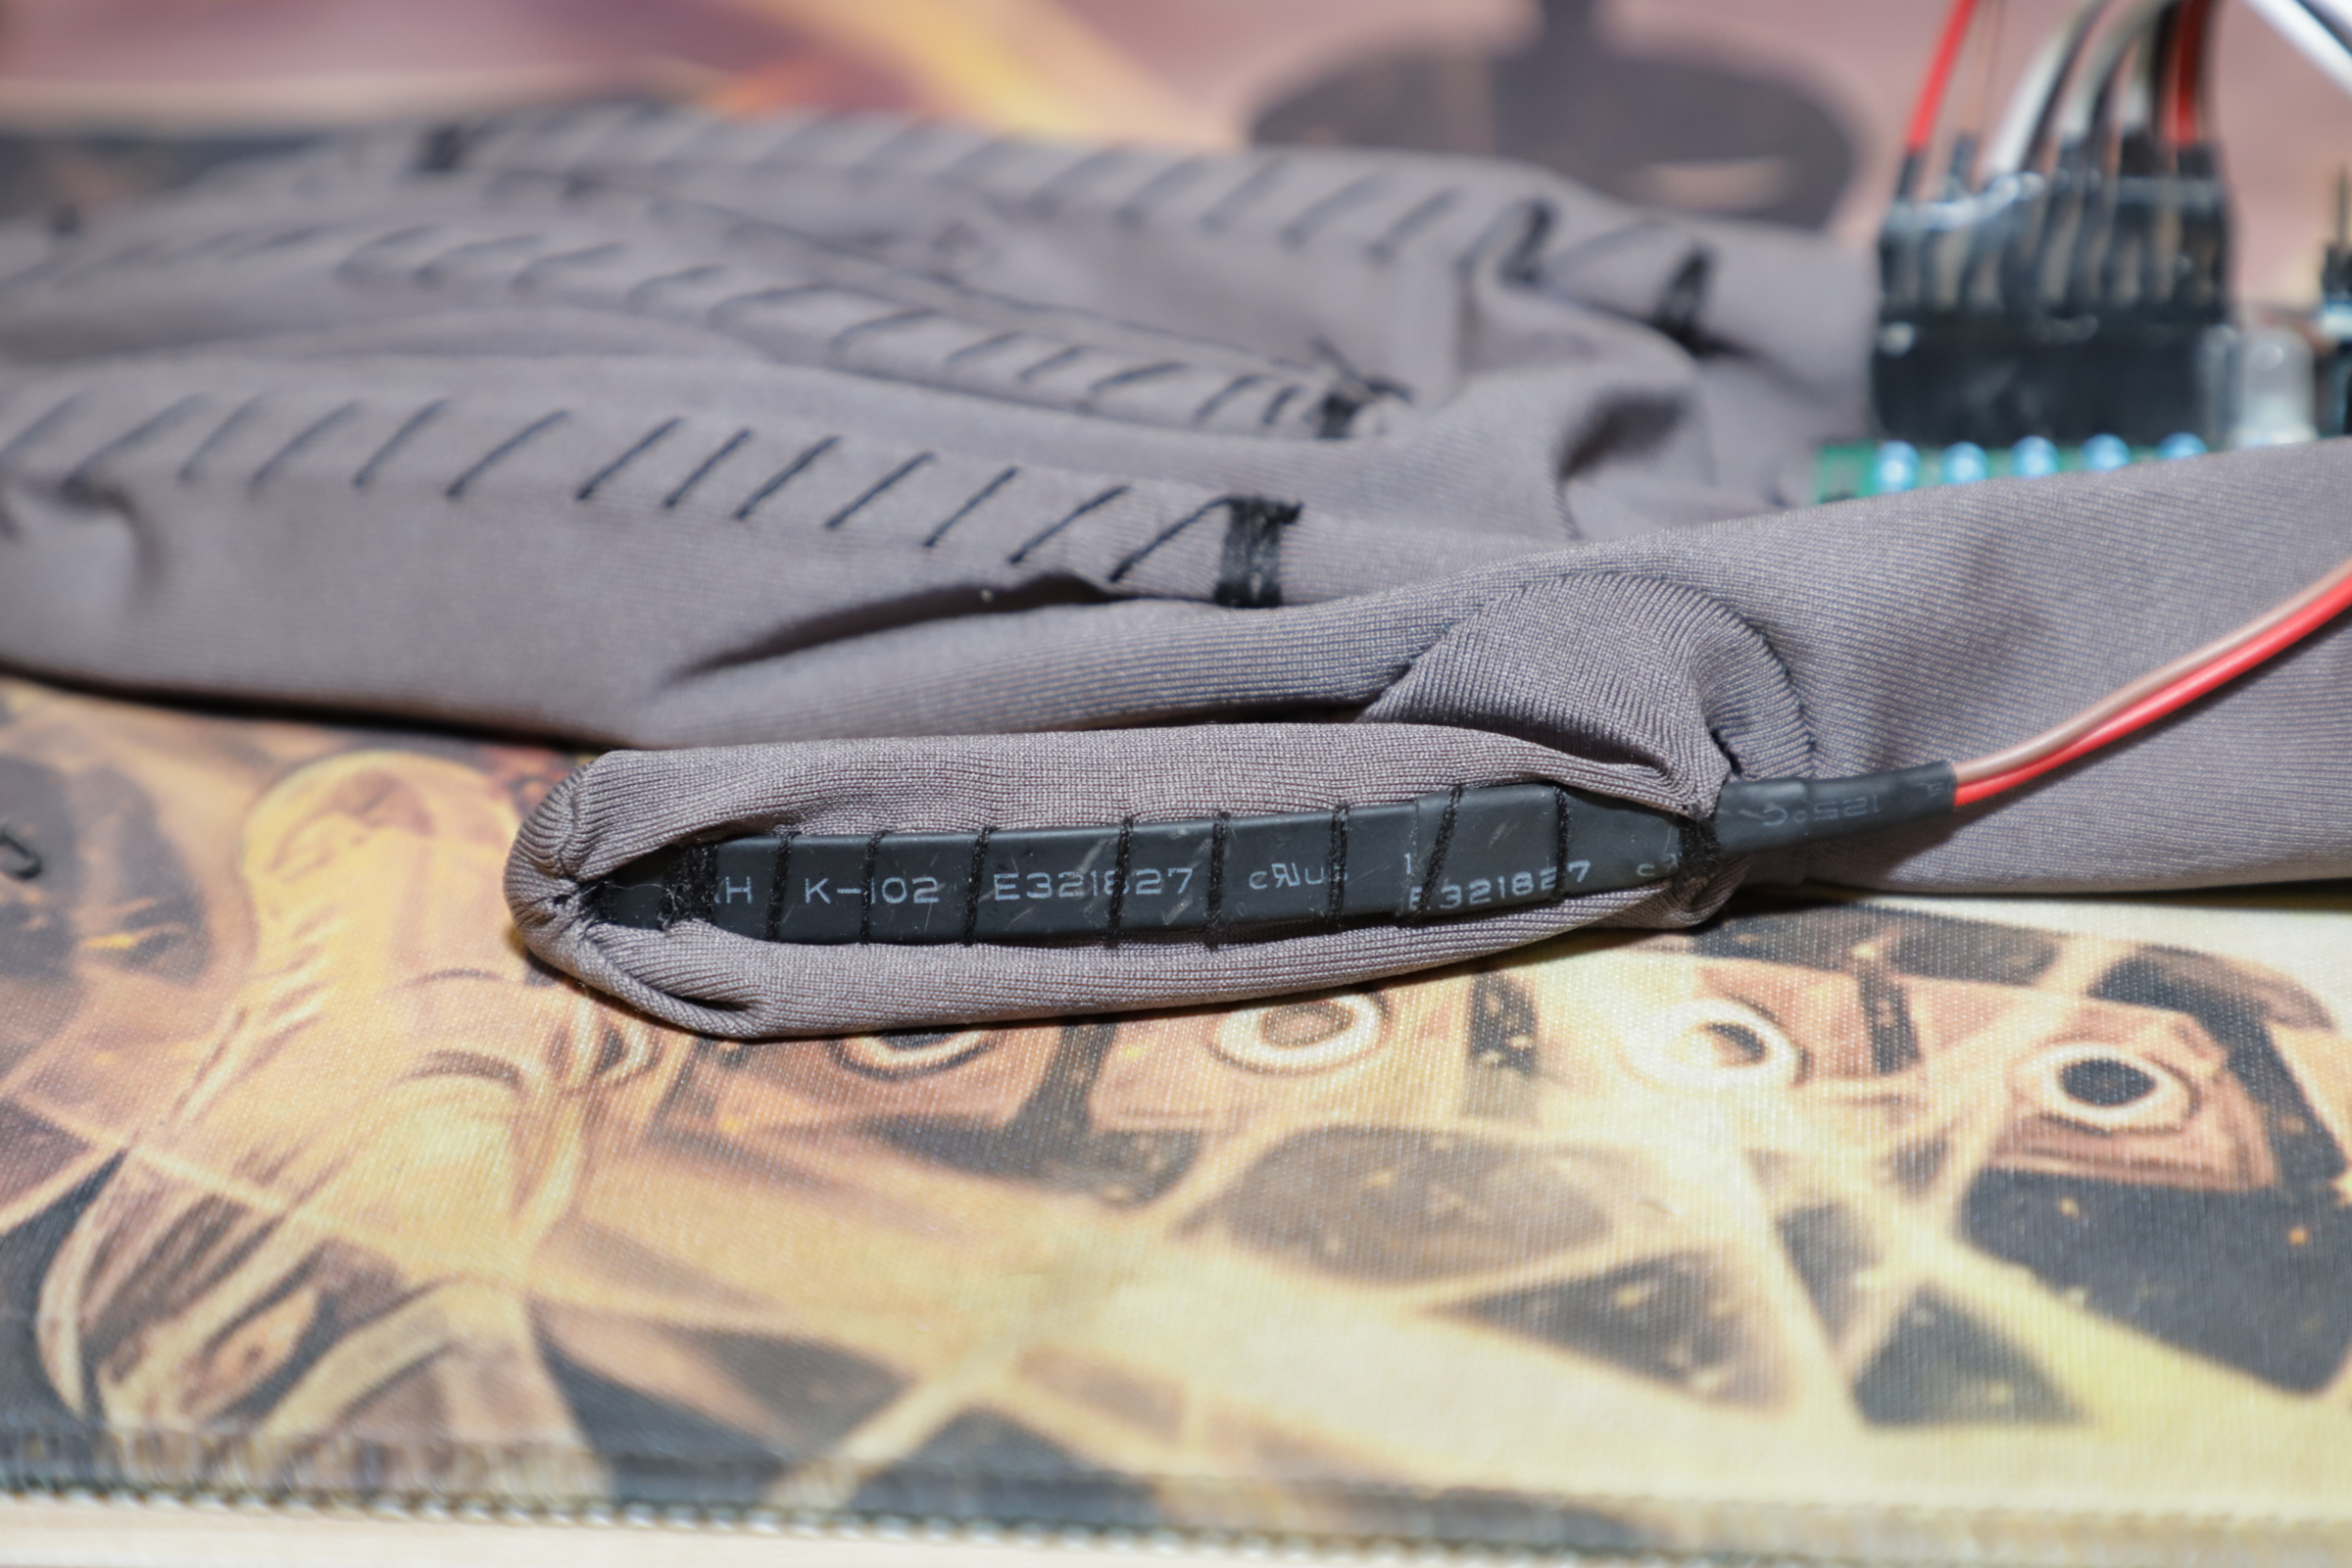
\includegraphics[width=10cm]{Images/Experimental results/flex_sensor.JPG}
\caption{Hình ảnh flex sensor trên sản phẩm}
\end{figure}

\indent Để thu thập và xử lý dữ liệu từ các cảm biến, chúng tôi tích hợp một bo mạch Arduino Nano, được đặt ngay ở mu bàn tay của bao tay. Arduino Nano đóng vai trò là bộ trung gian giữa cảm biến và gateway. Nó không chỉ thu thập dữ liệu từ các flex sensor mà còn có khả năng gửi dữ liệu đã xử lý đến gateway để chuẩn bị cho bước tiếp theo.

\begin{figure}[H]
    \centering
    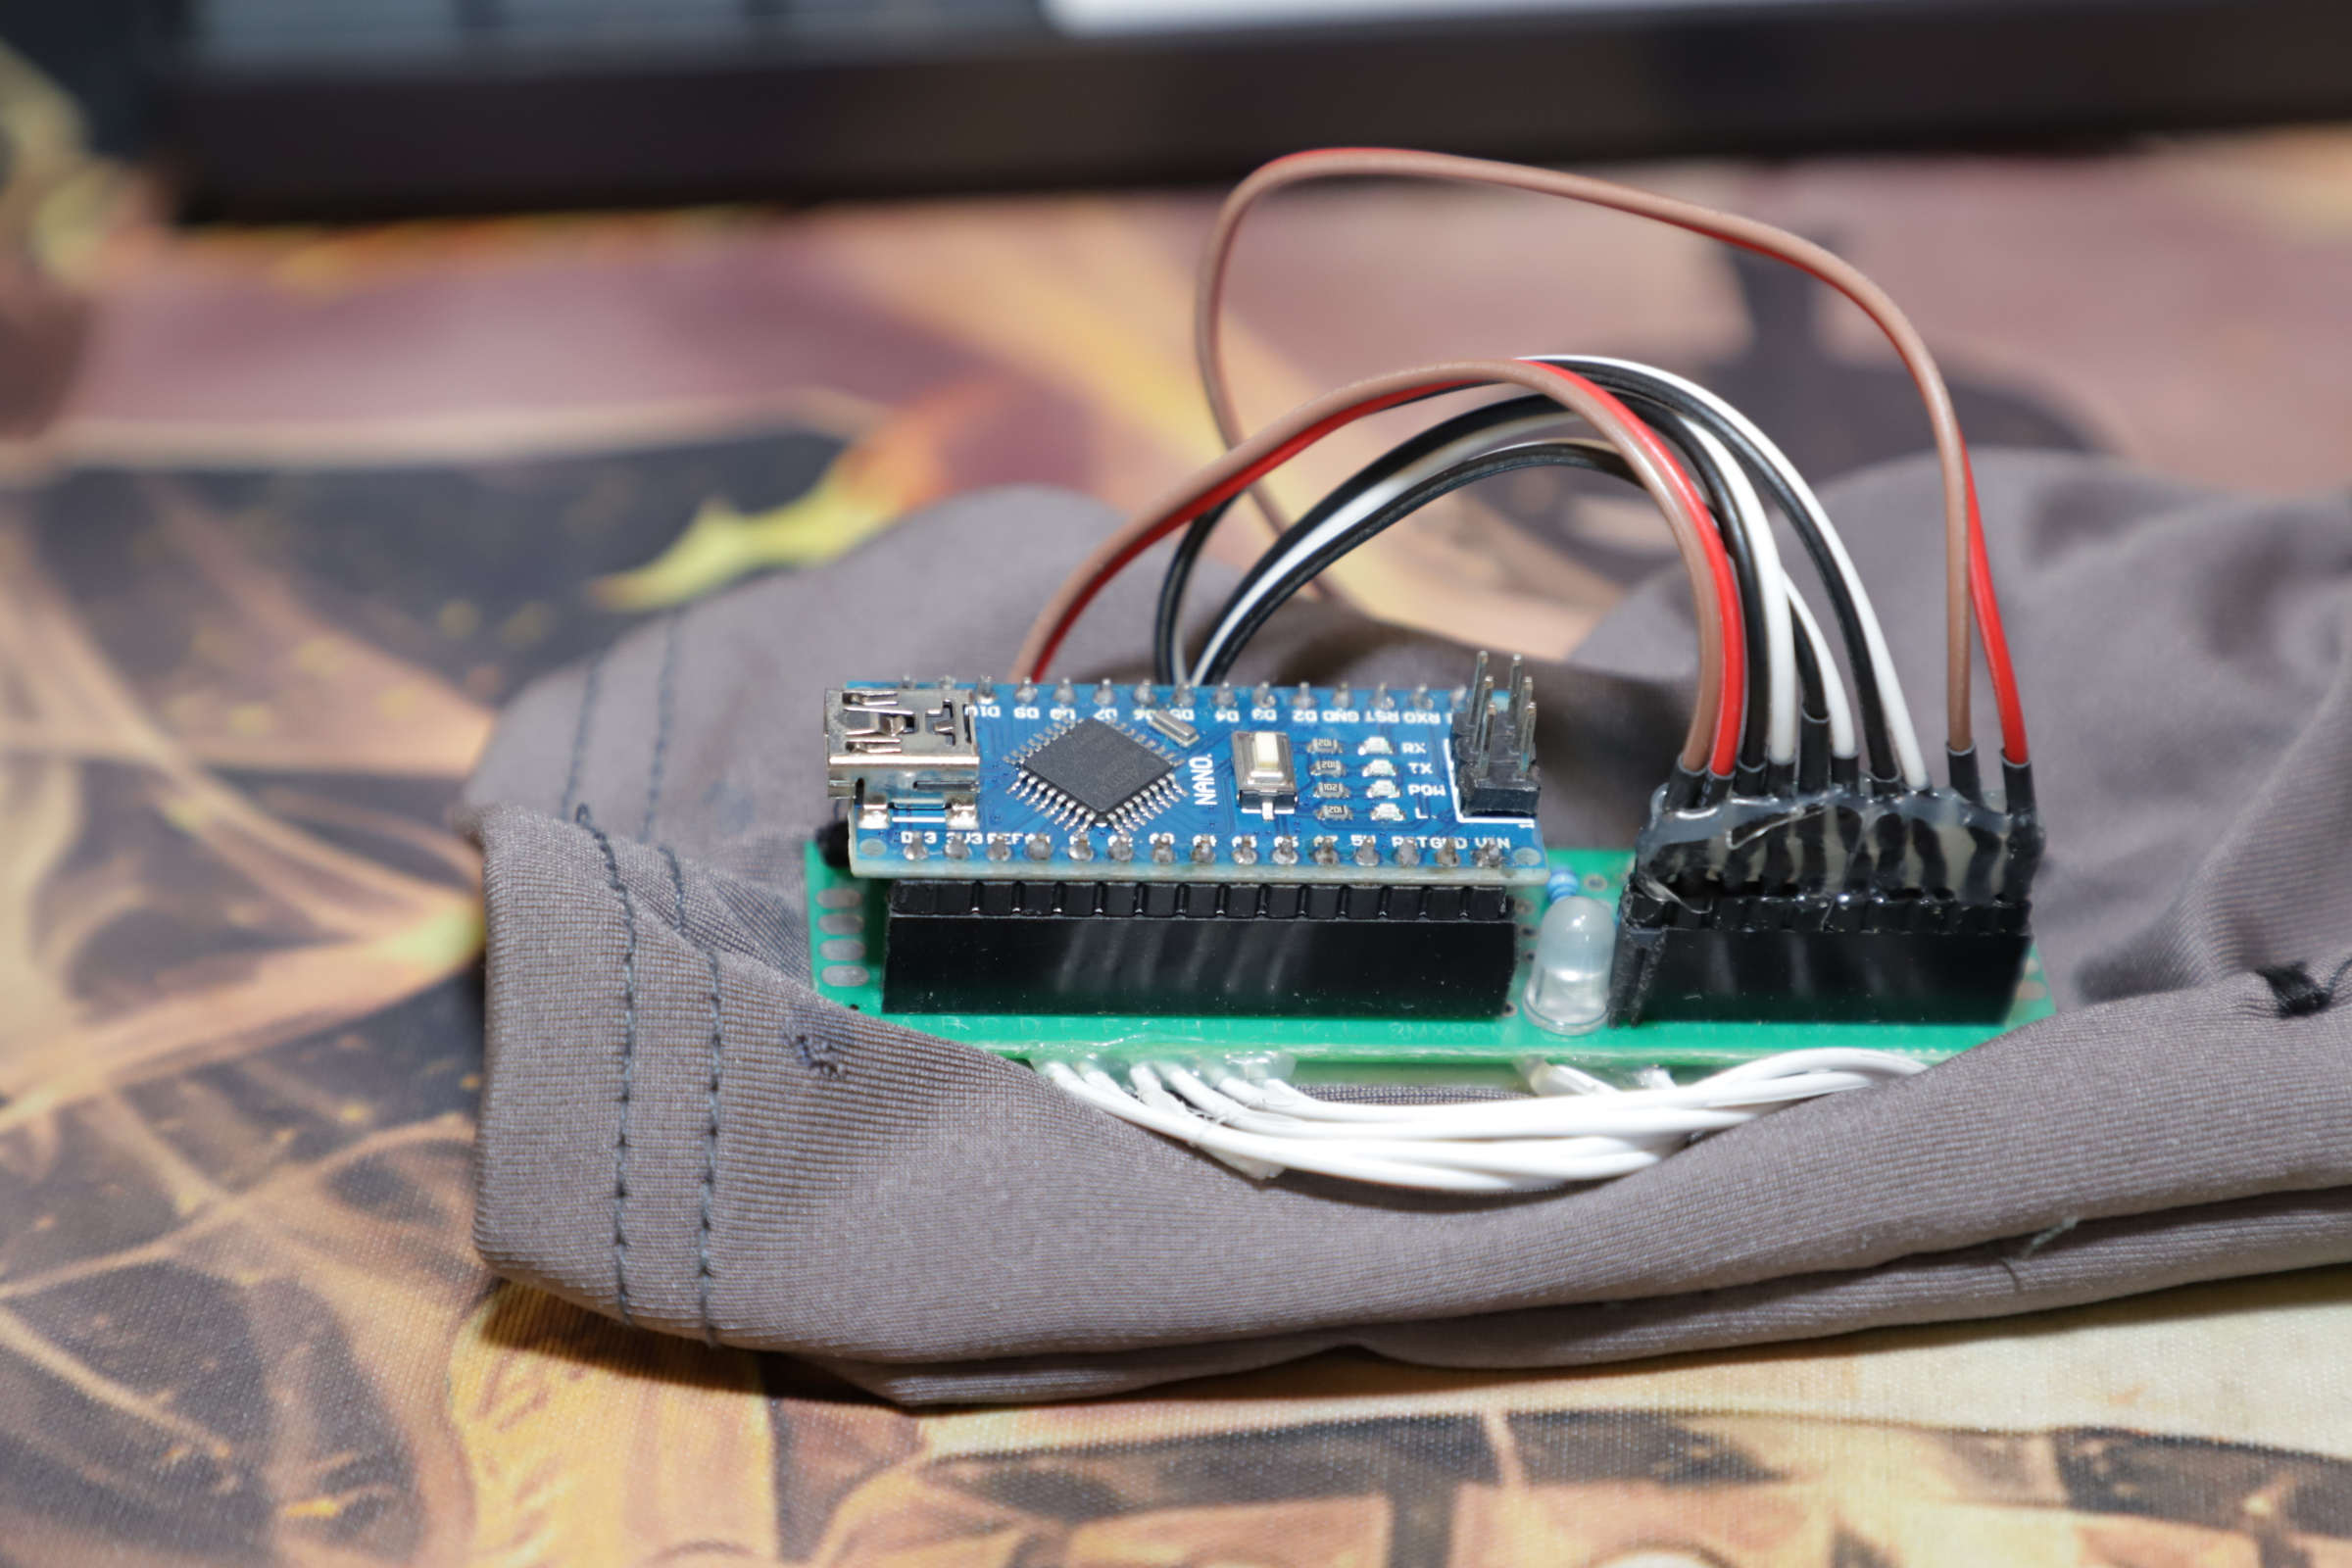
\includegraphics[width=13cm]{Images/Experimental results/arduino.JPG}
\caption{Hình ảnh arduino trên sản phẩm}
\end{figure}

\indent Kết quả đo đạc dữ liệu được minh họa trực quan thông qua biểu đồ trong video demo sau: \href{https://drive.google.com/file/d/15w1vhGEa1Rosjk0dPk62oQYnOiVk-edL/view?usp=drive_link}{Link Video Demo}

\indent Một số hình ảnh được cắt ra từ video:

\begin{figure}[H]
    \centering
    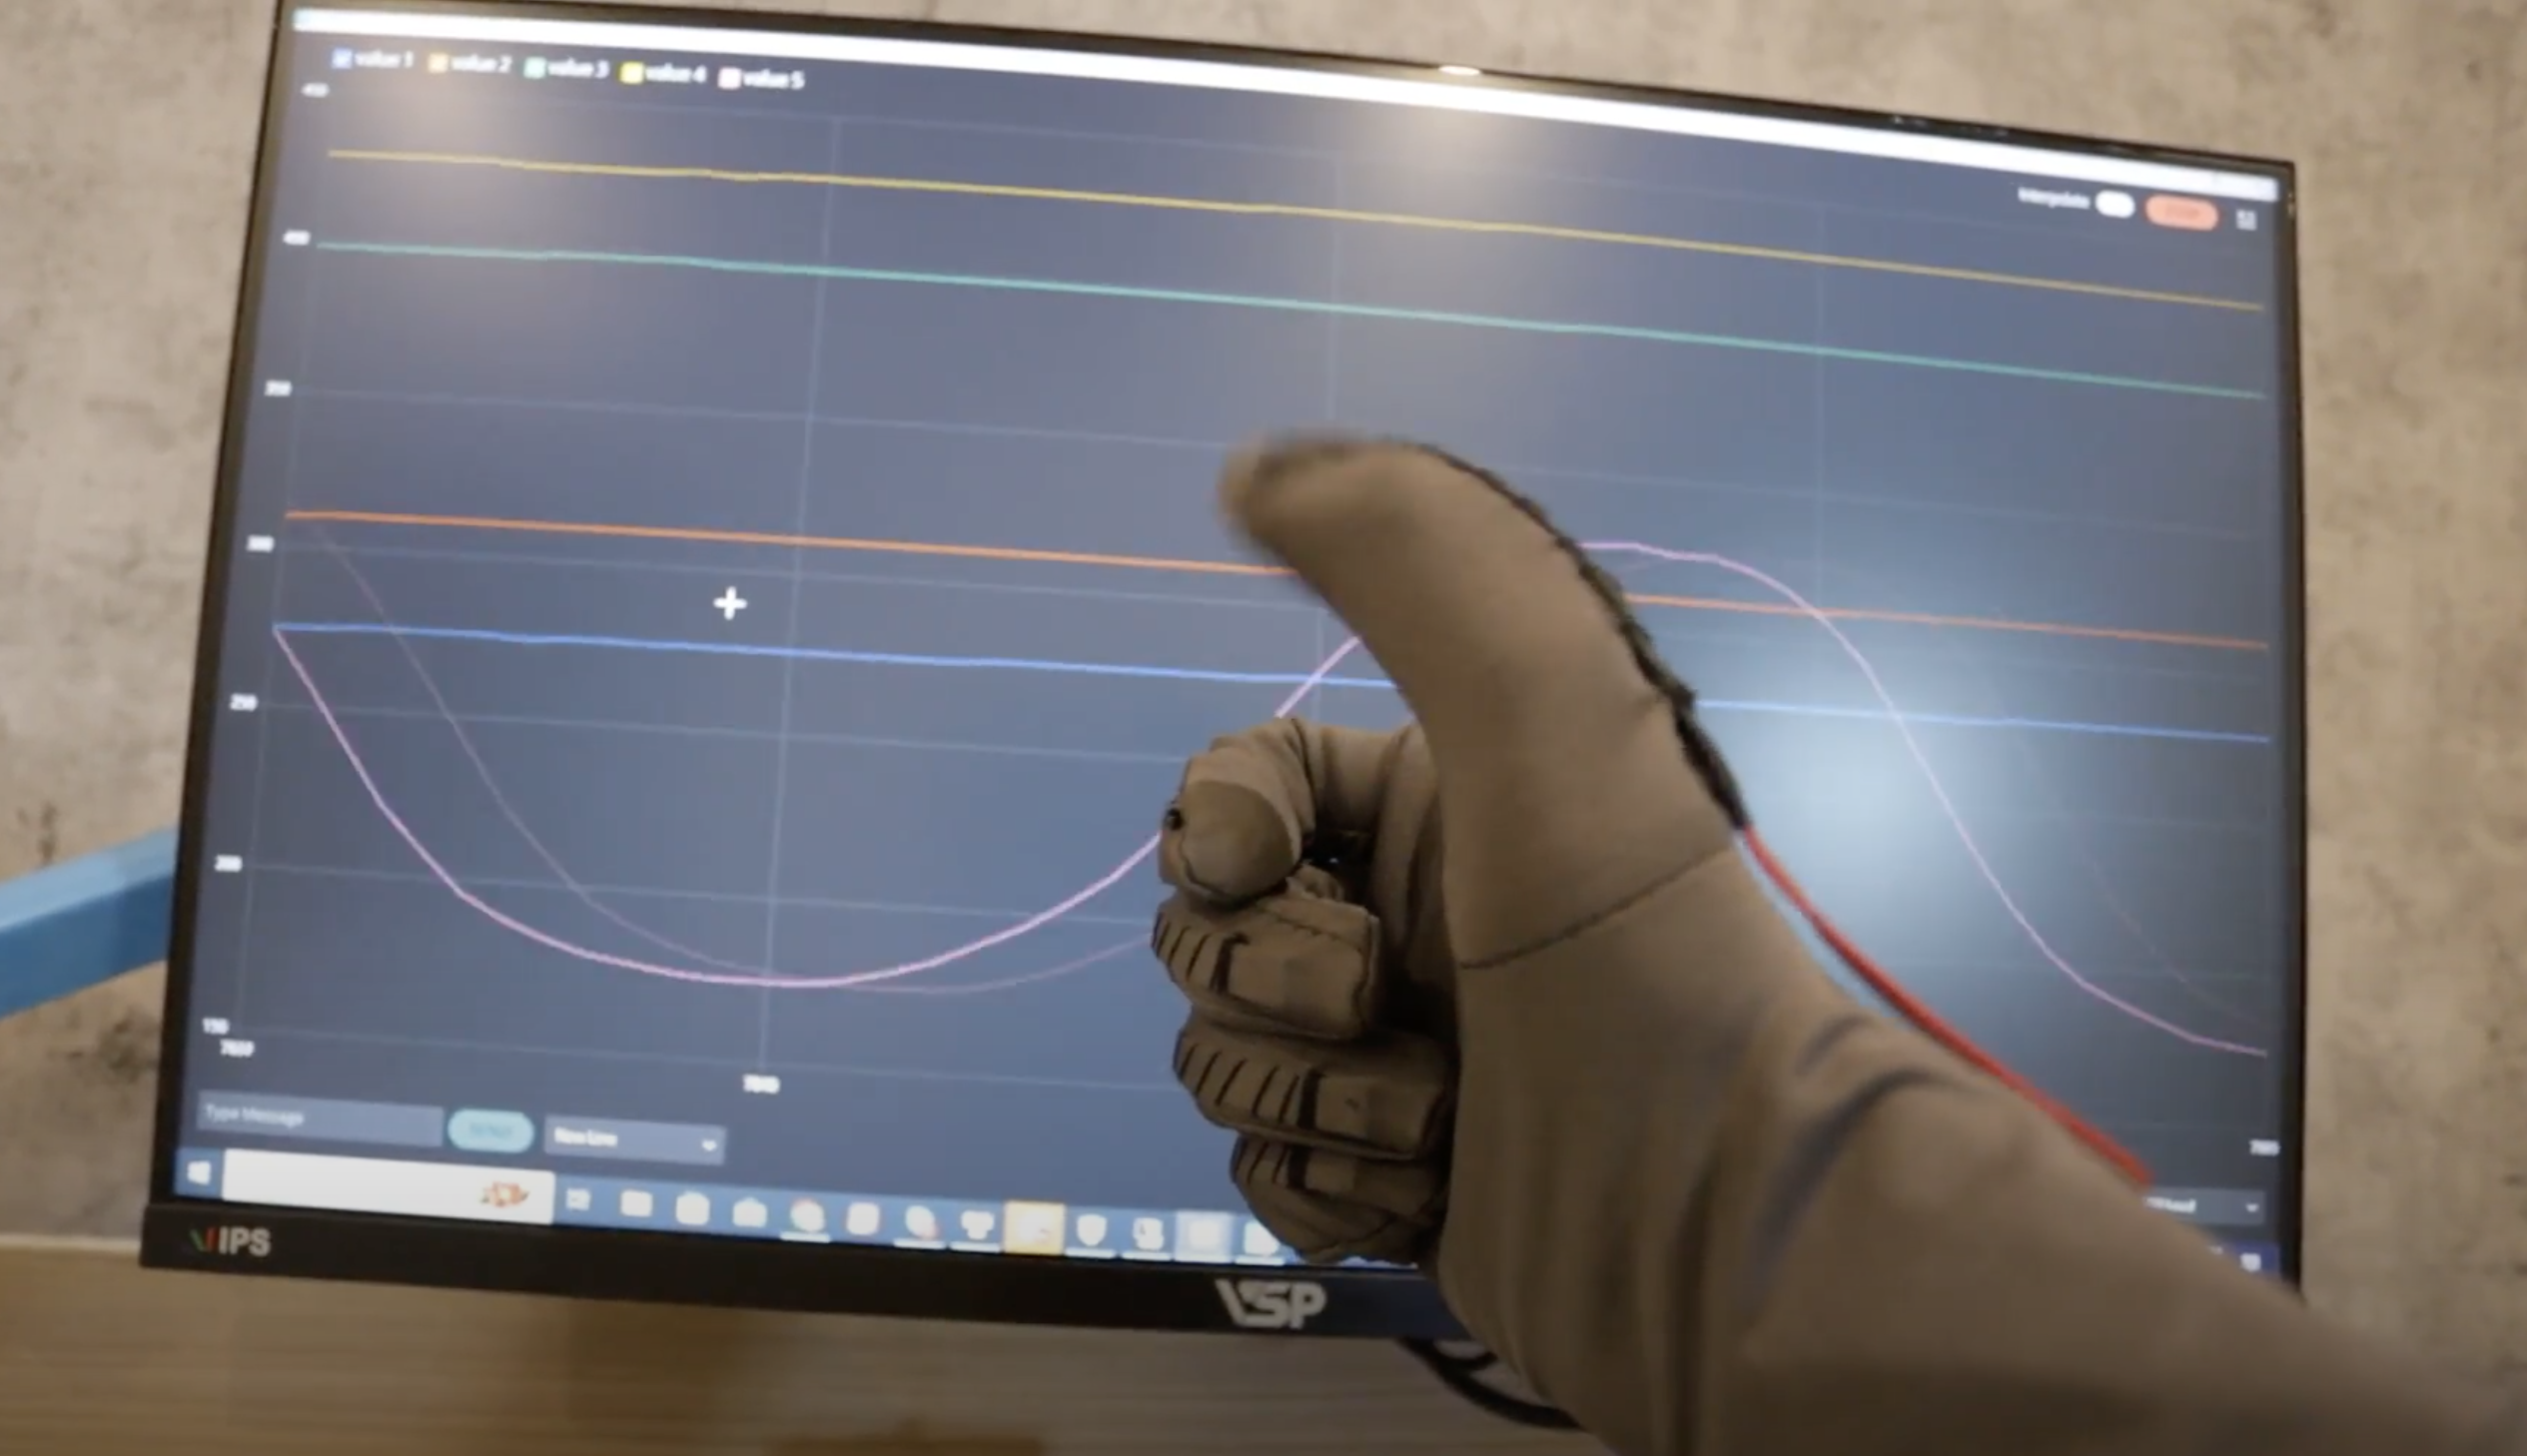
\includegraphics[width=10cm]{Images/Experimental results/readdt_result_1.png}
    
    \centering
    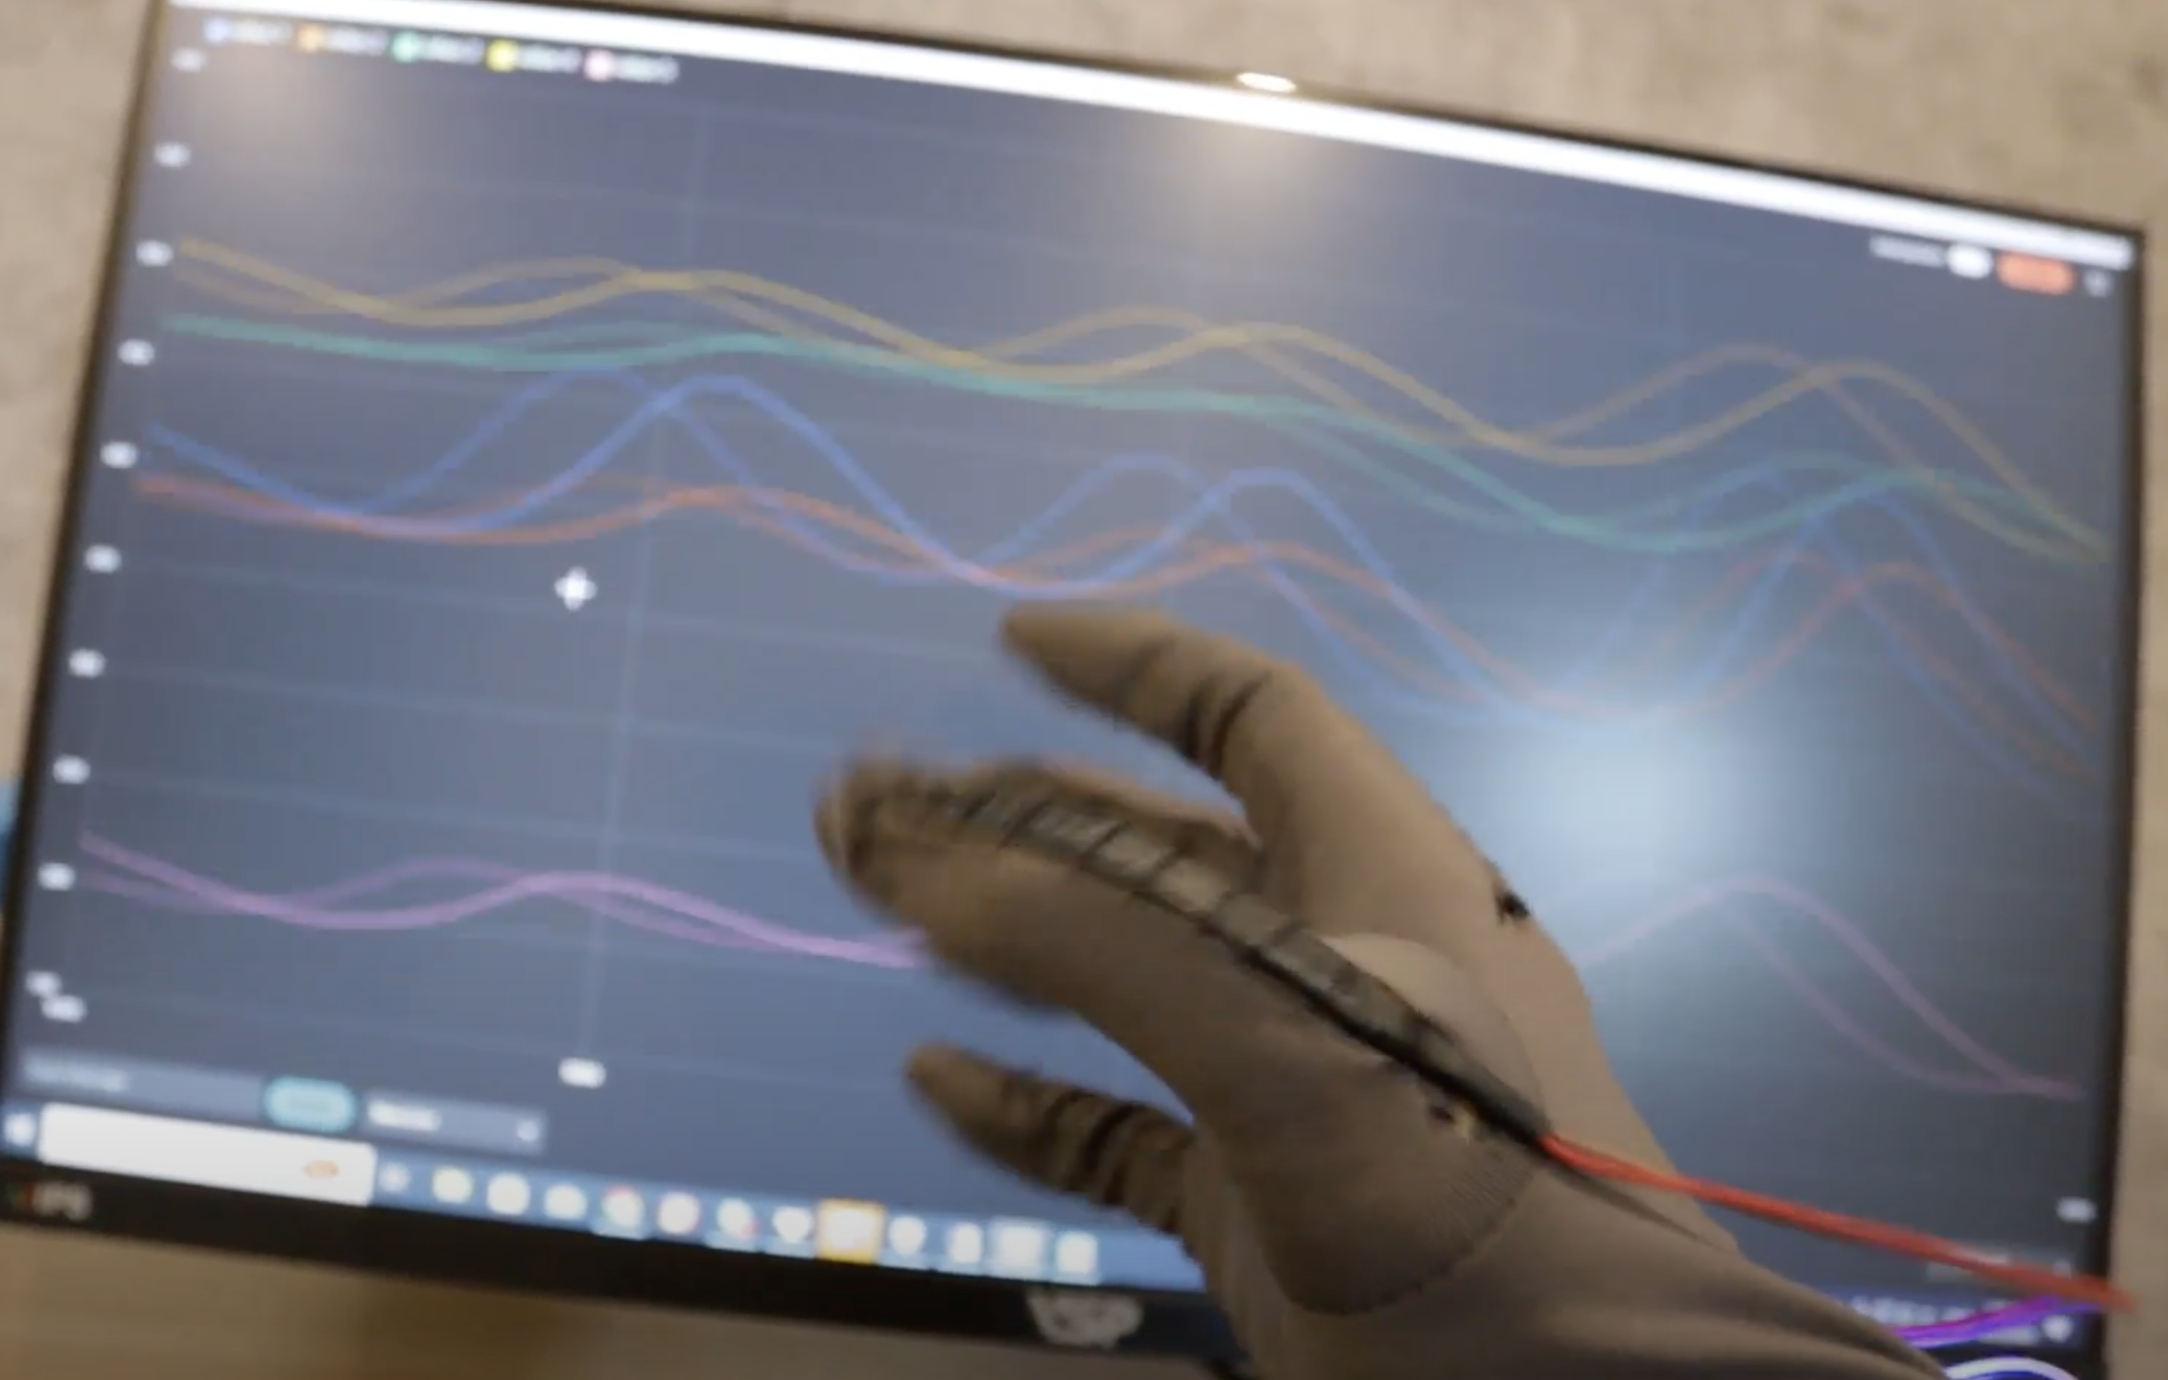
\includegraphics[width=10cm]{Images/Experimental results/readdt_result_2.png}
\caption{Quá trình lấy dữ liệu}
\end{figure}


\subsection{Mô hình LSTM}

\subsubsection{Mã nguồn}

\indent Mã nguồn này được thực thi trên gateway

\begin{lstlisting}
// cnn lstm model
from numpy import mean
from numpy import std
from numpy import dstack
from pandas import read_csv
from keras.models import Sequential
from keras.layers import Dense
from keras.layers import Flatten
from keras.layers import Dropout
from keras.layers import LSTM
from keras.layers import TimeDistributed
from keras.layers import Conv1D
from keras.layers import MaxPooling1D
from keras.utils import to_categorical
from matplotlib import pyplot
import time
// load a single file as a numpy array
def load_file(filepath):
	dataframe = read_csv(filepath, header=None, delim_whitespace=True)
	return dataframe.values

// load a list of files and return as a 3d numpy array
def load_group(filenames, prefix=''):
	loaded = list()
	for name in filenames:
		data = load_file(prefix + name)
		loaded.append(data)
	// stack group so that features are the 3rd dimension
	loaded = dstack(loaded)
	return loaded

// load a dataset group, such as train or test
def load_dataset_group(group, prefix=''):
	filepath = prefix + group + '/Inertial Signals/'
	// load all 9 files as a single array
	filenames = list()
	// total acceleration
	filenames += ['total_acc_x_'+group+'.txt', 'total_acc_y_'+group+'.txt', 'total_acc_z_'+group+'.txt']
	// body acceleration
	filenames += ['body_acc_x_'+group+'.txt', 'body_acc_y_'+group+'.txt', 'body_acc_z_'+group+'.txt']
	// body gyroscope
	filenames += ['body_gyro_x_'+group+'.txt', 'body_gyro_y_'+group+'.txt', 'body_gyro_z_'+group+'.txt']
	// load input data
	X = load_group(filenames, filepath)
	// load class output
	y = load_file(prefix + group + '/y_'+group+'.txt')
	return X, y

// load the dataset, returns train and test X and y elements
def load_dataset(prefix=''):
	// load all train
	trainX, trainy = load_dataset_group('train', prefix + 'HARDataset/')
	print('train', prefix + 'HARDataset/')
	print(trainX.shape, trainy.shape)
	// load all test
	testX, testy = load_dataset_group('test', prefix + 'HARDataset/')
	print('test', prefix + 'HARDataset/')
	print(testX.shape, testy.shape)
	// zero-offset class values
	trainy = trainy - 1
	testy = testy - 1
	// one hot encode y
	trainy = to_categorical(trainy)
	testy = to_categorical(testy)
	print(trainy)
	print(testy)
	print('------------------------------------------------')
	print(trainX.shape, trainy.shape, testX.shape, testy.shape)
	return trainX, trainy, testX, testy

// fit and evaluate a model
def evaluate_model(trainX, trainy, testX, testy):
	// define model
	verbose, epochs, batch_size = 0, 25, 64
	n_timesteps, n_features, n_outputs = trainX.shape[1], trainX.shape[2], trainy.shape[1]
	print(n_timesteps)
	// reshape data into time steps of sub-sequences
	n_steps, n_length = 4, 32
	trainX = trainX.reshape((trainX.shape[0], n_steps, n_length, n_features))
	testX = testX.reshape((testX.shape[0], n_steps, n_length, n_features))
	print(trainX.shape)
	print(testX.shape)
	// define model
	model = Sequential()
	model.add(TimeDistributed(Conv1D(filters=64, kernel_size=3, activation='relu'), input_shape=(None,n_length,n_features)))
	model.add(TimeDistributed(Conv1D(filters=64, kernel_size=3, activation='relu')))
	model.add(TimeDistributed(Dropout(0.5)))
	model.add(TimeDistributed(MaxPooling1D(pool_size=2)))
	model.add(TimeDistributed(Flatten()))
	model.add(LSTM(100))
	model.add(Dropout(0.5))
	model.add(Dense(100, activation='relu'))
	model.add(Dense(n_outputs, activation='softmax'))
	model.compile(loss='categorical_crossentropy', optimizer='adam', metrics=['accuracy'])
	// fit network
	model.fit(trainX, trainy, epochs=epochs, batch_size=batch_size, verbose=verbose)
	// evaluate model
	_, accuracy = model.evaluate(testX, testy, batch_size=batch_size, verbose=0)
	yhat = model.predict(testX, verbose=0)
	i_str = 0
	inputs = input('integer')
	while inputs:
		time.sleep(0.1)
		i_str += 1
		
		// Check if the input is empty (user pressed Enter without typing anything)
		if not i_str or i_str > 2946:
			break
		
		try:
			i = int(i_str)
			result = yhat[i]
			rounded_result = [round(num, 1) for num in result]  // Round each number to three decimal places
			print('result is', rounded_result)
		except ValueError:
			print('Please enter a valid integer.')

	return accuracy

// summarize scores
def summarize_results(scores):
	print(scores)
	m, s = mean(scores), std(scores)
	print('Accuracy: %.3f%% (+/-%.3f)' % (m, s))

// run an experiment
def run_experiment(repeats=1):
	// load data
	trainX, trainy, testX, testy = load_dataset()
	// repeat experiment
	scores = list()
	for r in range(repeats):
		score = evaluate_model(trainX, trainy, testX, testy)
		score = score * 100.0
		print('>//%d: %.3f' % (r+1, score))
		scores.append(score)
	// summarize results
	summarize_results(scores)

// run the experiment
run_experiment()
\end{lstlisting}
\subsubsection{Mô tả bộ dữ liệu}
\indent Dữ liệu của mô hình trên được sử dụng từ bài báo LSTMs for Human Activity Recognition Time Series Classification vì tính khả thi và phù hợp với đề tài

\indent Thông Tin Về Thí Nghiệm: 

\indent 30 tình nguyện viên trong khoảng độ tuổi 19-48 tham gia. Mỗi người thực hiện sáu hoạt động (Đi bộ, Đi bộ Lên Cầu Thang, Đi bộ Xuống Cầu Thang, Ngồi, Đứng, Nằm) với việc đeo một smartphone (Samsung Galaxy S II) ở vùng eo.

\indent Sử dụng cảm biến gia tốc và gyroscope tích hợp, ghi lại gia tốc tuyến tính 3 trục và vận tốc góc 3 trục với tần suất 50Hz.
Thực hiện quay video để gán nhãn dữ liệu một cách thủ công.

\indent Bộ dữ liệu được chia ngẫu nhiên thành hai phần, với 70\% tình nguyện viên được chọn để tạo dữ liệu huấn luyện và 30\% làm dữ liệu kiểm thử.

\indent Tiền Xử Lý Dữ Liệu:

\indent Tín hiệu cảm biến (accelerometer và gyroscope) được tiền xử lý bằng cách áp dụng bộ lọc nhiễu.

\indent Dữ liệu được chia thành cửa sổ trượt có độ dài cố định là 2.56 giây và chồng lấn 50\% (128 đọc/giây).

\indent Tín hiệu gia tốc, có thành phần trọng lực và chuyển động cơ thể, được tách bằng bộ lọc thấp Butterworth thành gia tốc cơ thể và trọng lực.

\indent Từ mỗi cửa sổ, thu được một vector đặc trưng bằng cách tính toán biến từ miền thời gian và tần số. Xem 'features\_info.txt' để biết thêm chi tiết.

\indent Thông Tin về Mỗi Bản Ghi gồm:
\begin{itemize}

\item Gia tốc 3 trục từ accelerometer (gia tốc tổng) và gia tốc cơ thể ước lượng.

\item Vận tốc góc 3 trục từ gyroscope.

\item Một vector đặc trưng có 561 biến từ miền thời gian và tần số.

\item Nhãn hoạt động.

\item Một định danh của người tham gia thí nghiệm.

\item Các Tệp Dữ Liệu:

'activity\_labels.txt': Liên kết nhãn lớp với tên hoạt động.

'train/X\_train.txt': Tập huấn luyện.

'train/y\_train.txt': Nhãn huấn luyện.

'test/X\_test.txt': Tập kiểm thử.

'test/y\_test.txt': Nhãn kiểm thử.

\end{itemize}

\subsubsection{Mô tả cách tải và xử lí dữ liệu}

Bước đầu tiên là tải dữ liệu gốc vào bộ nhớ.


Có ba loại tín hiệu chính trong dữ liệu gốc: gia tốc tổng, gia tốc cơ thể và gyroscope cơ thể. Mỗi loại có 3 trục dữ liệu. Điều này có nghĩa là tổng cộng có chín biến số cho mỗi bước thời gian. Hơn nữa, mỗi loạt dữ liệu đã được chia thành các cửa sổ chồng lấn của 2.56 giây dữ liệu, tương đương với 128 bước thời gian. Các cửa sổ dữ liệu này tương ứng với các cửa sổ đặc trưng đã được tạo ra trước đó. Điều này có nghĩa là một hàng dữ liệu có (128 * 9), tức là 1,152 phần tử.\\


Các tín hiệu được lưu trữ trong thư mục /Inertial Signals/ dưới các thư mục con train và test. Mỗi trục của mỗi tín hiệu được lưu trữ trong một tệp riêng biệt, có nghĩa là mỗi bộ dữ liệu train và test có 9 tệp đầu vào để tải và một tệp đầu ra để tải. Có thể tải các tệp này thành các nhóm dựa trên cấu trúc thư mục và quy ước đặt tên tệp nhất quán.\\


Dữ liệu đầu vào được định dạng dưới dạng CSV trong đó các cột được phân tách bằng khoảng trắng. Mỗi tệp này có thể được tải như một mảng NumPy. Hàm load\_file() tải một bộ dữ liệu dựa trên đường dẫn đầy đủ đến tệp và trả về dữ liệu đã tải như một mảng NumPy. Chúng ta có thể sau đó tải tất cả dữ liệu cho một nhóm cụ thể (huấn luyện hoặc kiểm thử) vào một mảng NumPy ba chiều duy nhất, trong đó kích thước của mảng là [mẫu, bước thời gian, đặc trưng].\\


Để làm cho điều này rõ ràng hơn, có 128 bước thời gian và chín đặc trưng, với số mẫu là số hàng trong bất kỳ tệp dữ liệu tín hiệu gốc nào. Hàm load\_group() thực hiện hành vi này. Hàm dstack() của NumPy cho phép  xếp từng mảng 3D đã tải vào một mảng 3D duy nhất trong đó các biến được phân tách trên chiều thứ ba (đặc trưng).
Có thể sử dụng hàm này để tải tất cả dữ liệu tín hiệu đầu vào cho một nhóm cụ thể, chẳng hạn như huấn luyện hoặc kiểm thử. \\


Hàm load\_dataset\_group() tải tất cả dữ liệu tín hiệu đầu vào và dữ liệu đầu ra cho một nhóm duy nhất sử dụng các quy ước đặt tên nhất quán giữa các thư mục.\\


Cuối cùng,có thể tải mỗi tập dữ liệu huấn luyện và kiểm thử. Dữ liệu đầu ra được định nghĩa dưới dạng số nguyên cho số lớp. Chúng ta cần mã hóa one-hot cho các số nguyên lớp này để dữ liệu phù hợp để đào tạo một mô hình phân loại đa lớp sử dụng mạng nơ-ron. Chúng ta có thể thực hiện điều này bằng cách gọi hàm to\_categorical() trong Keras. Hàm load\_dataset() thực hiện hành vi này và trả về các phần X và y của tập huấn luyện và kiểm thử đã sẵn sàng để đào tạo và đánh giá các mô hình được định nghĩa.

\subsubsection{Mô tả mô hình}

Bây giờ khi đã tải dữ liệu vào bộ nhớ để chuẩn bị cho mô hình hóa, ta có thể định nghĩa, đào tạo và đánh giá một mô hình LSTM.\\

Có thể định nghĩa một hàm có tên là evaluate\_model() nhận bộ dữ liệu huấn luyện và kiểm thử, đào tạo mô hình trên tập dữ liệu huấn luyện, đánh giá nó trên tập dữ liệu kiểm thử và trả về ước lượng về hiệu suất của mô hình.\\

Trước hết, phải định nghĩa mô hình LSTM bằng thư viện học sâu Keras. Mô hình yêu cầu một đầu vào ba chiều với [mẫu, bước thời gian, đặc trưng]. Điều này chính xác như cách chúng ta đã tải dữ liệu, nơi một mẫu là một cửa sổ của dữ liệu chuỗi thời gian, mỗi cửa sổ có 128 bước thời gian và một bước thời gian có chín biến số hoặc đặc trưng.\\

Đầu ra cho mô hình sẽ là một vector sáu phần tử chứa xác suất của một cửa sổ cụ thể thuộc về mỗi trong sáu loại hoạt động. Các kích thước đầu vào và đầu ra này là bắt buộc khi đào tạo mô hình, và chúng ta có thể trích xuất chúng từ tập dữ liệu huấn luyện đã cung cấp.\\

Mô hình được định nghĩa như một mô hình tuần tự Sequential của Keras, vì sự đơn giản.\\

Tiếp đến sẽ định nghĩa mô hình có một lớp ẩn LSTM duy nhất. Sau đó là một lớp dropout nhằm giảm overfitting của mô hình với dữ liệu huấn luyện. Cuối cùng, sử dụng một lớp kết nối đầy đủ để giải thích các đặc trưng được trích xuất bởi lớp ẩn LSTM, trước khi sử dụng lớp đầu ra cuối cùng để đưa ra dự đoán.\\

Tiếp đến sẽ sử dụng phiên bản hiệu quả Adam giảm độ dốc để tối ưu hóa mạng, và hàm mất mát entropy chéo phân loại hạng mục sẽ được sử dụng vì đang phân loại đa lớp.\\

Mô hình được đào tạo trong một số epoch cố định, trong trường hợp này là 15, và một kích thước batch là 64 mẫu sẽ được sử dụng, trong đó 64 cửa sổ dữ liệu sẽ được mô hình tiếp xúc trước khi trọng số của mô hình được cập nhật.\\

Khi mô hình đã được đào tạo, nó sẽ được đánh giá trên tập dữ liệu kiểm thử và độ chính xác của mô hình đã đào tạo trên tập dữ liệu kiểm thử sẽ được trả về.\\

Lưu ý, thông thường là không cần phải xáo trộn dữ liệu chuỗi khi đào tạo một LSTM. Trong trường hợp này, thực hiện việc xáo trộn các cửa sổ dữ liệu đầu vào trong quá trình đào tạo (mặc định). Trong vấn đề này quan tâm đến khả năng của LSTM để học và trích xuất đặc trưng qua các bước thời gian trong một cửa sổ, không phải qua các cửa sổ.\\


\subsubsection{Kết quả hiện thực }
\indent Kết quả được hiển thị dứoi dạng one-hot-code để thể hiện được cả độ chính xác và kết quả đầu ra.

\begin{lstlisting}
.
.
.
result is [0.0, 0.0, 0.0, 0.4, 0.6, 0.0]
result is [0.0, 0.0, 0.0, 0.3, 0.7, 0.0]
result is [0.0, 0.0, 0.0, 0.3, 0.7, 0.0]
result is [0.0, 0.0, 0.0, 0.3, 0.7, 0.0]
result is [0.0, 0.0, 0.0, 0.3, 0.7, 0.0]
result is [0.0, 0.0, 0.0, 0.2, 0.8, 0.0]
result is [0.0, 0.0, 0.0, 0.0, 1.0, 0.0]
result is [0.0, 0.0, 0.0, 0.0, 1.0, 0.0]
.
.
.
\end{lstlisting}

\indent Kết quả đầu ra được thể hiện dưới dạng one-hot-code, ví dụ hàng 1 được dự đoán nhãn 4 và 5 với độ chính xác lần lượt là 40\% và 60\%, hàng 2 được dự đoán nhãn 4 và 5 lần lượt là 30\% và 70\% và tương tự cho các hàng còn lại


\subsubsection{Tóm tắt kết quả }

Chúng ta không thể đánh giá kỹ năng của mô hình chỉ từ một lần đánh giá.\\

Nguyên nhân là mạng nơ-ron là ngẫu nhiên, có nghĩa là một cấu hình mô hình cụ thể khác nhau sẽ xuất hiện khi đào tạo cùng một cấu hình mô hình trên cùng một dữ liệu.\\

Điều này là một đặc trưng của mạng, vì nó mang lại khả năng thích ứng cho mô hình, nhưng yêu cầu một quá trình đánh giá mô hình phức tạp hơn.\\

Chúng ta sẽ lặp lại việc đánh giá mô hình nhiều lần, sau đó tóm tắt hiệu suất của mô hình qua từng lần chạy đó. Ví dụ, chúng ta có thể gọi hàm evaluate\_model() tổng cộng 10 lần. Điều này sẽ dẫn đến một tập hợp các điểm đánh giá mô hình cần được tóm tắt.'\\

\begin{lstlisting}
>#1: 90.058
>#2: 85.918
>#3: 90.974
>#4: 89.515
>#5: 90.159
>#6: 91.110
>#7: 89.718
>#8: 90.295
>#9: 89.447
>#10: 90.024

[90.05768578215134, 85.91788259246692, 90.97387173396675, 89.51476077366813, 90.15948422124194, 91.10960298608755, 89.71835765184933, 90.29521547336275, 89.44689514760775, 90.02375296912113]

Accuracy: 89.722% (+/-1.371)

\end{lstlisting}
Cuối cùng, mẫu các điểm đánh giá được in ra, tiếp theo là giá trị trung bình và độ lệch chuẩn. Chúng ta có thể thấy rằng mô hình đã hoạt động tốt, đạt được độ chính xác phân loại khoảng 89,7\% khi được huấn luyện trên dữ liệu thô, với độ lệch chuẩn là khoảng 1,3. Đây là một kết quả tốt ! 








